\chapter{Product Architecture}

\section{Systems Overview} 
The alpha prototype is composed of three major systems: the propulsion arm system, the landing leg system and the control electronics system. The 3 main systems work in unison to transform an amateur rocket into a full fledged autonomous landing system capable of deploying the necessary components and safely landing the rocket. Each of these primary systems is composed of an array of smaller components that work in unison to perform the systems required tasks for safe landing. A full CAD assembly of the final design without the upper airframe is shown in Figure \ref{arch:full-cad:labelled}
\begin{figure}[H]
    \centering
    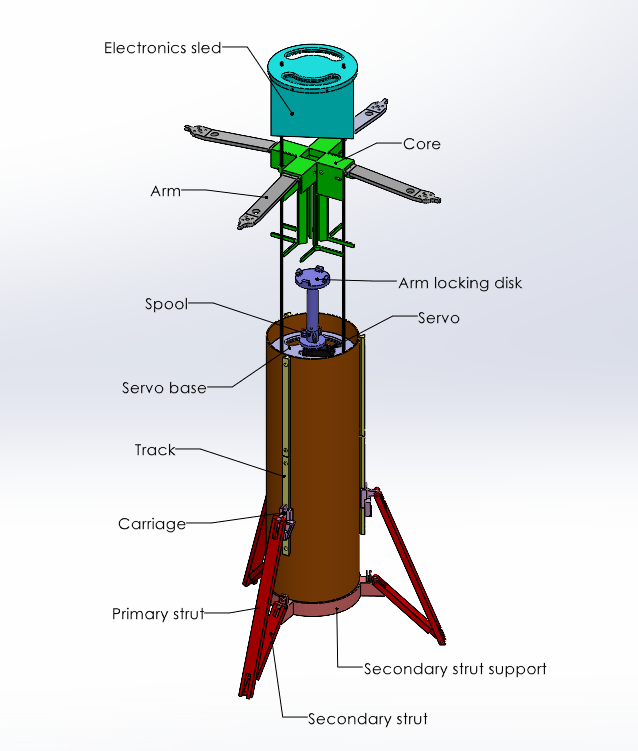
\includegraphics[width=\textwidth]{src/figs/full-labelled-cad-assembly.png}
    \caption{Full labelled CAD assembly without upper airframe}
    \label{arch:full-cad:labelled}
\end{figure}

\section{Control System Electronics Functionality}
The control system electronics are responsible for detecting whether the rocket is falling, deploying the propulsion arms and landing legs, and autonomous stabilization and navigation of the rocket. This system is composed of the Pixhawk flight controller which is responsible for running ArduPilot firmware for flight stabilization, a Raspberry Pi 4 model B flight computer which is used for running Python scripts for autonomous missions, an IMU for measuring acceleration, a radio transmitter for communicating with the QGroundControl groundstation application, electronic speed controllers for motor control, a 3S LiPo battery for the motors, and a separate rechargeable battery for the Raspberry Pi. A power distribution board is used to get power to all of the components. Images of the front and back of the avionics bay are shown in figures \ref{fig:AVF} and \ref{fig:AVB}.

\begin{figure}[H]
    \centering
    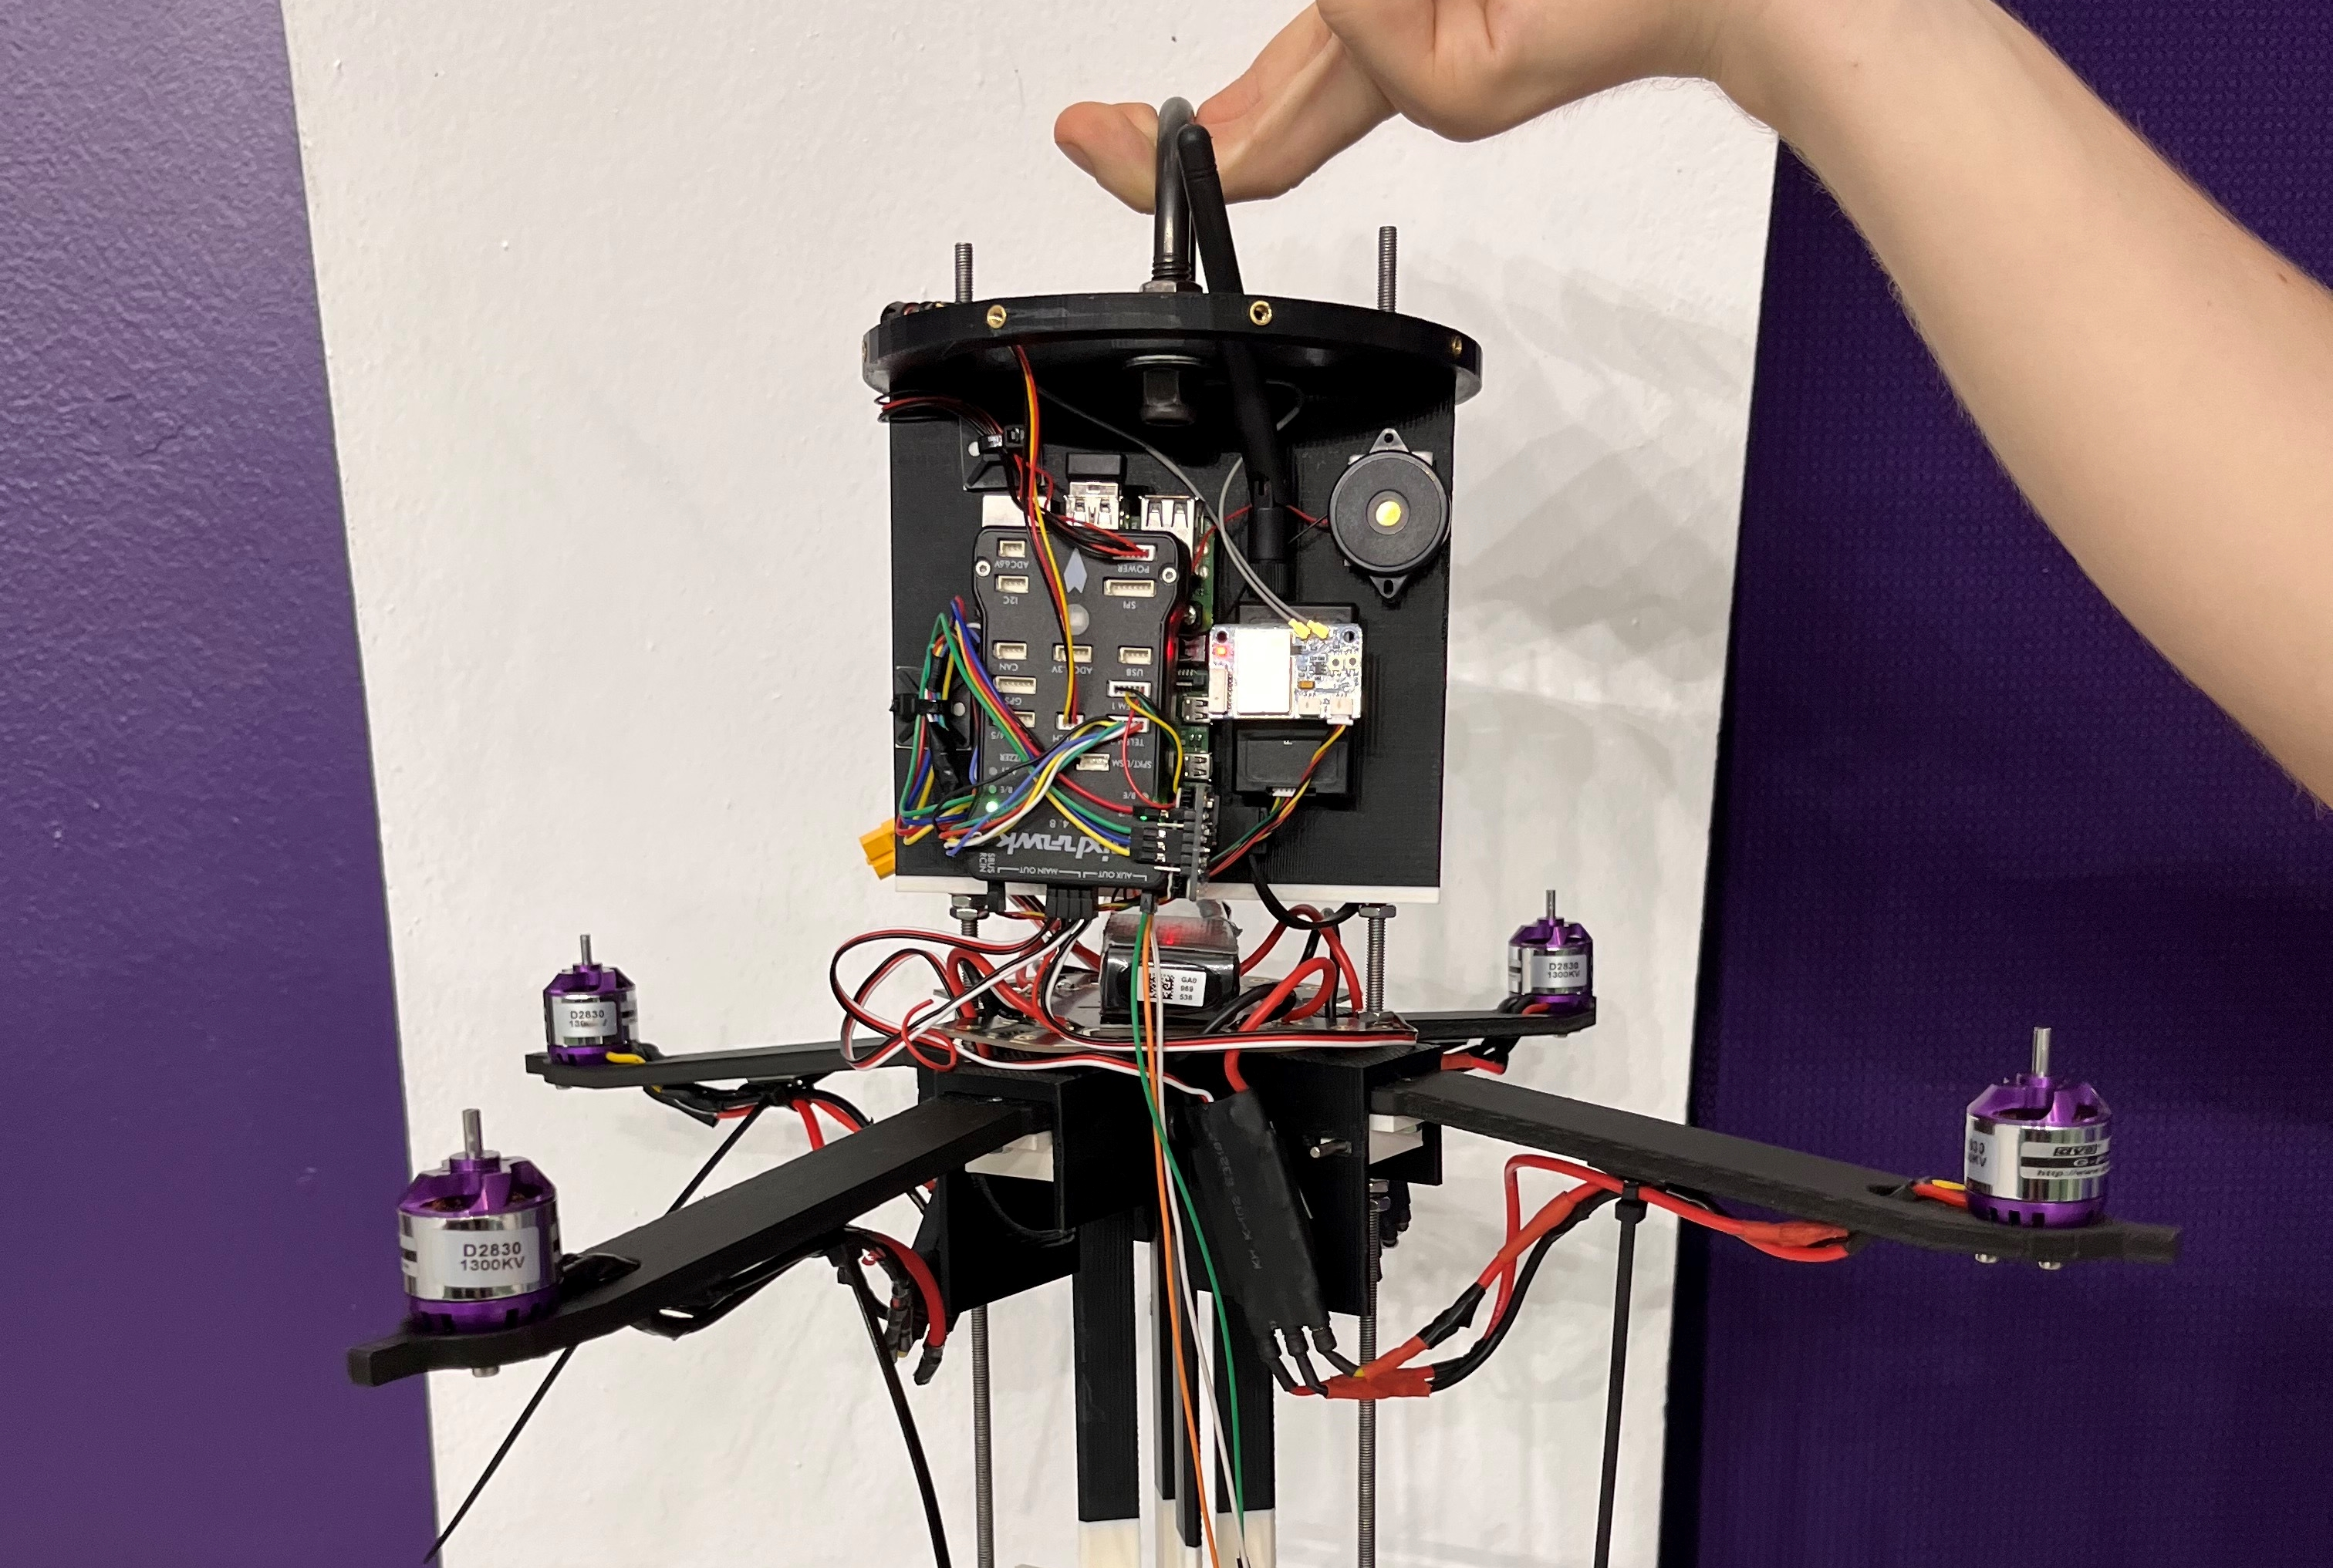
\includegraphics[width=\textwidth]{src/figs/AVBay_Front.jpg}
    \caption{Avionics Bay Front}
    \label{fig:AVF}
\end{figure}

\begin{figure}[H]
    \centering
    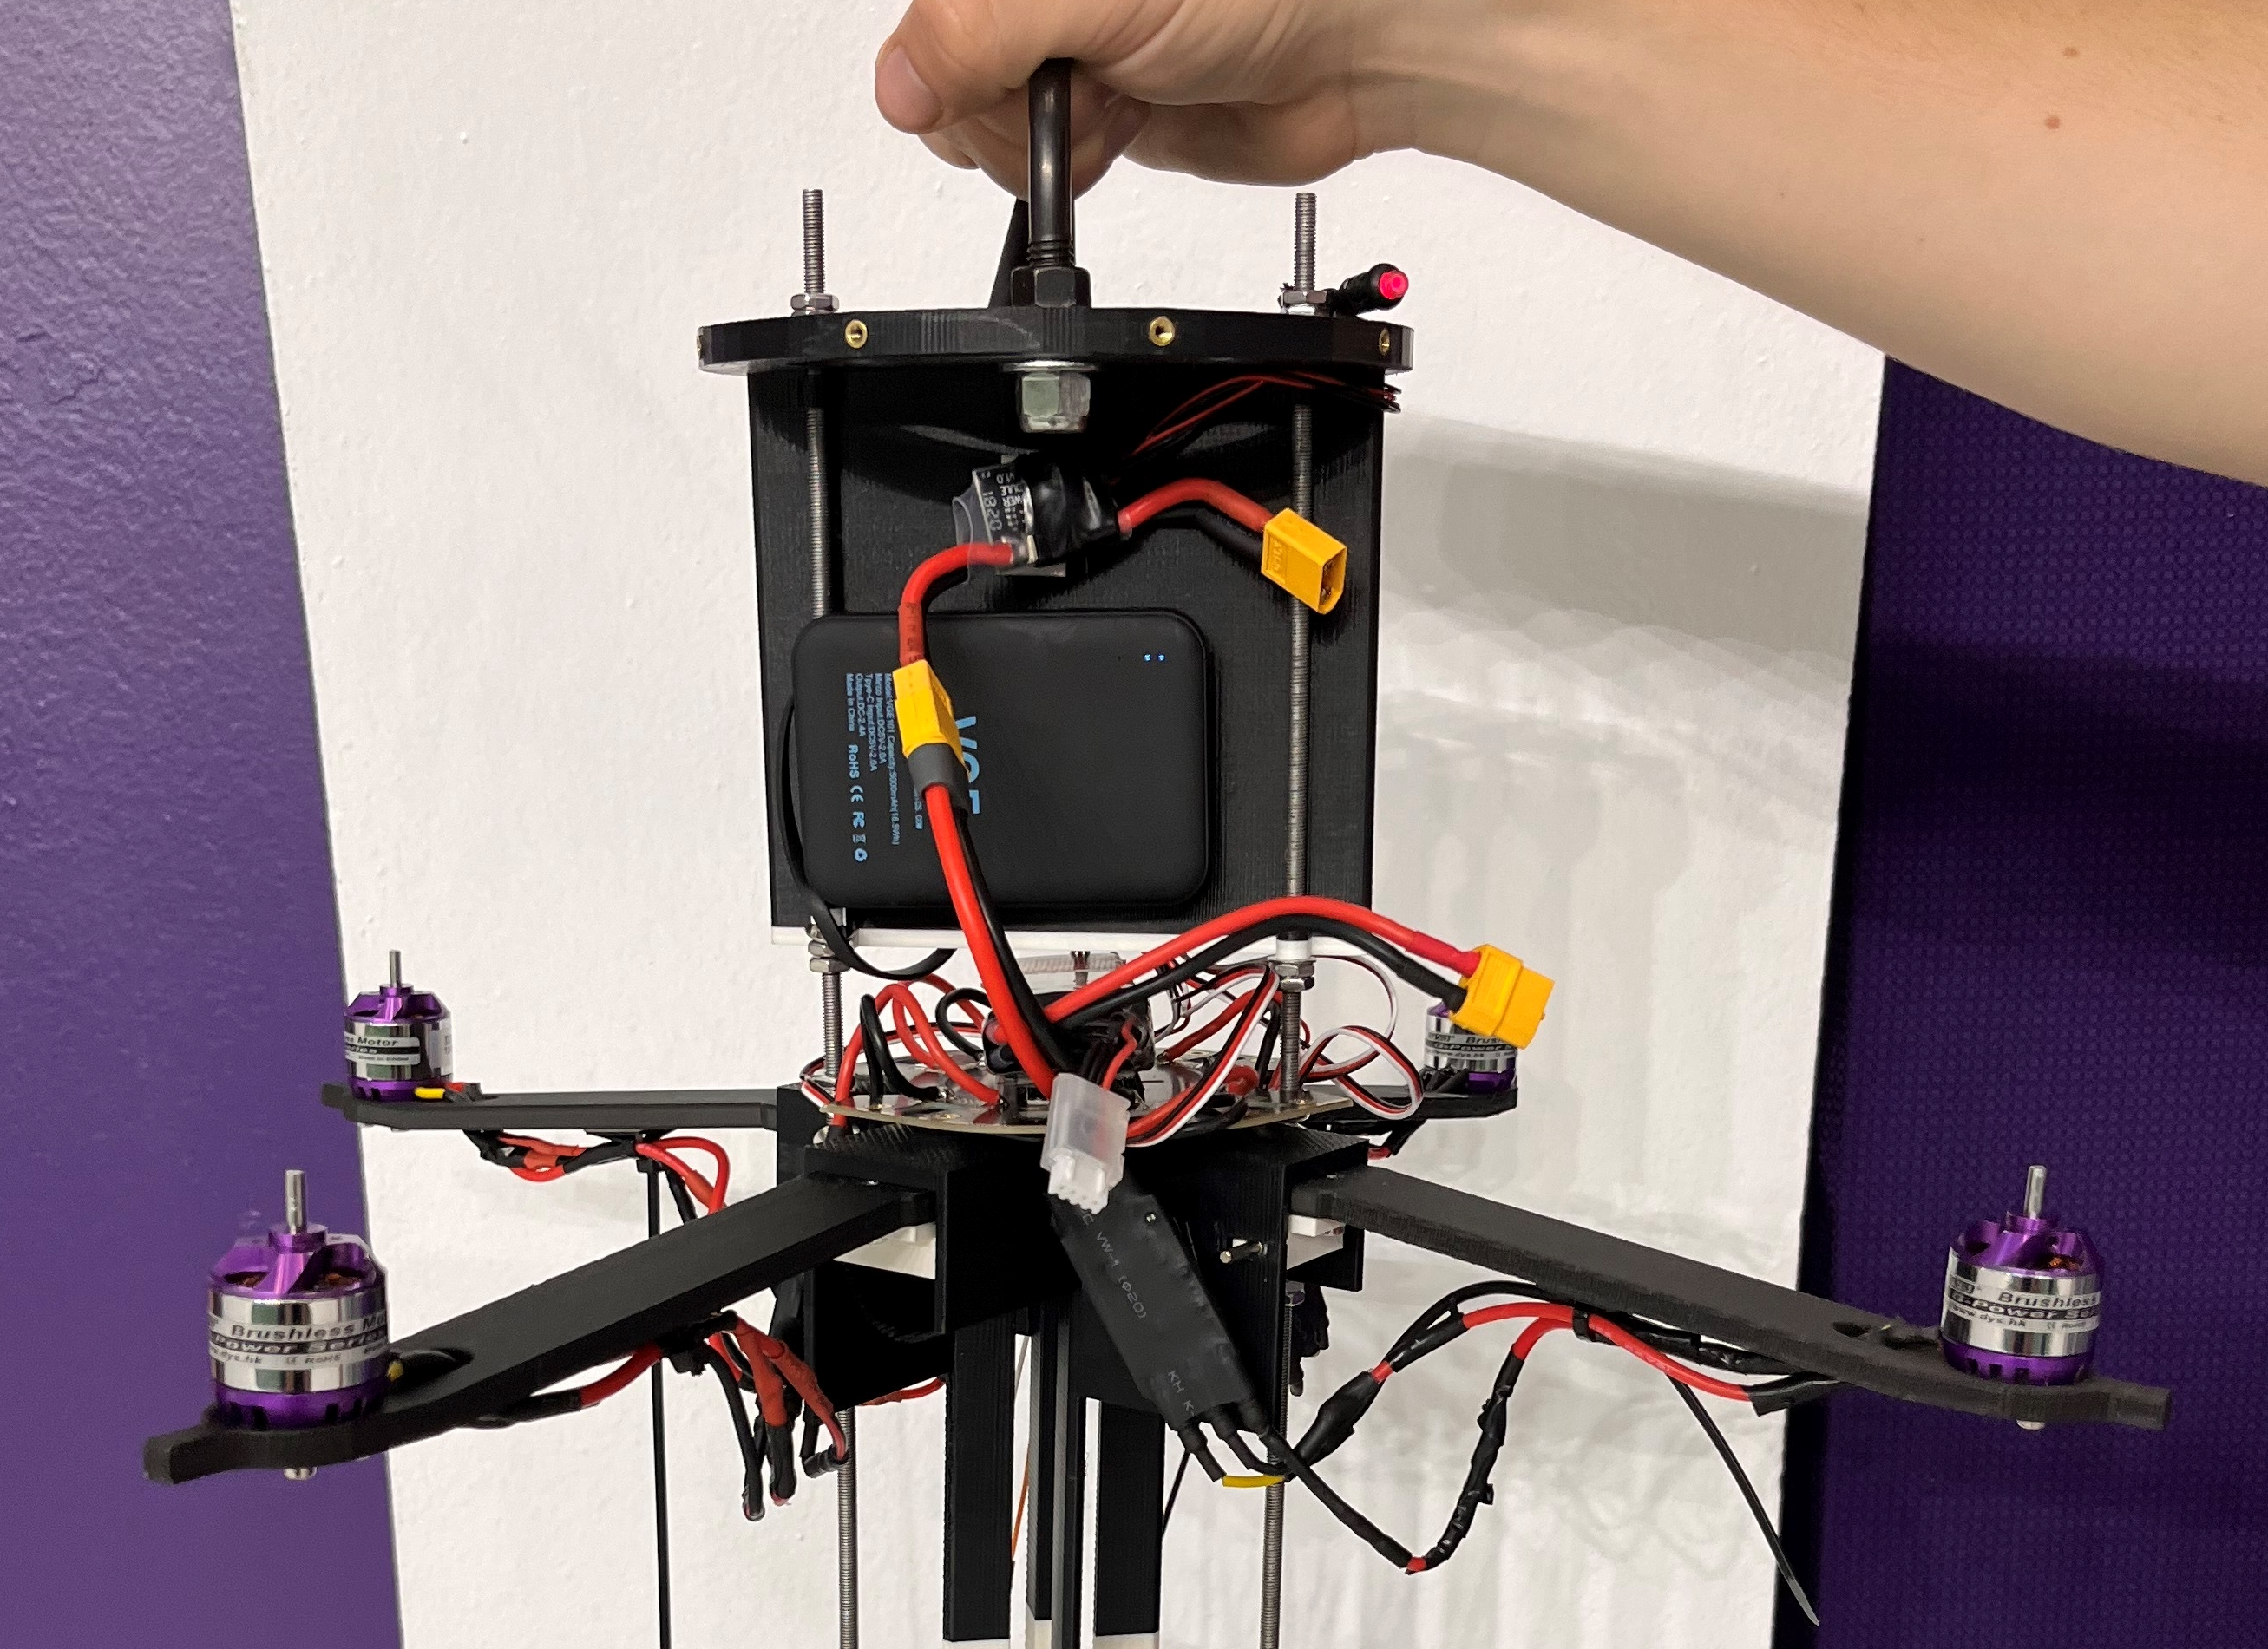
\includegraphics[width=\textwidth]{src/figs/AVBay_Back.jpg}
    \caption{Avionics Bay Back}
    \label{fig:AVB}
\end{figure}




\section{Propulsion Arm System Functionality}
The propulsion arm system is responsible for supporting the necessary components for lift generation as well as the components required to stow and deploy the system from the rocket body. The main component of this system is the propulsion arm which is solely responsible for providing a platform to which the motor mounts to and attaching to the rocket. The system is composed of 4 propulsion arms, each with an identical set of supporting components. The design of the arm was heavily driven by the development and design of these supporting components which are discussed below. The entire arm assembly will be explain and shown in figures in the following subsection.


\subsection{Upper and Lower Support Plates}
To simplify the assembly and maintenance procedures for the system, all components were designed to be modular and easy to remove from the rocket body. To facilitate this design requirement, two 10/32 aluminum threaded rods are vertically oriented on the inside of the rocket body. These rods are attached at their ends to two support plates which attach to the rocket body via 16 threaded inserts and accompanying M3 screws. The upper support plate has an extrusion below it that provides a flat mounting surface for a large portion of the control electronics. These are mounted above the propulsion arms in an effort to balance the moment caused by the landing legs to maintain the rockets center of mass as close to the center of thrust as possible.

\subsection{Deployment Method}
Each propulsion arm deploys through the use of two torsion springs which attach to the underside of the arm. When stowed, these springs are in their compressed position and actively trying to push the propulsion arms outside of the rocket body. Since the full travel from fully stowed to fully deployed for each of the arms is 90 degrees, torsion springs with a 120 degree free angle were selected to prevent over compression of the spring. To prevent premature deployment of the arms, a pre-deployment locking mechanism was developed that could simultaneously deploy all four arms on command.

\subsection{Pre-Deployment Locking Mechanism}
The pre-deployment locking mechanism is composed of a disk that rotates on command via a servo connected to it. The servo is recessed into the lower support plate via an interference fit cutout. It is then further secured to the plate via two bolts and nuts to prevent movement in the event of an unusual flight attitude. 

The disk has four protrusions or 'tabs' that are spaced every 90 degrees. These tabs interface with the arm when it is stowed in order to hold it inside the rocket body. Upon command, the disk rotates and the tabs are no longer aligned with the stowed arms allowing them to deploy to their operational position outside the rocket body. This all is shown in figure \ref{fig:stowedarm}.

\begin{figure}[H]
    \centering
    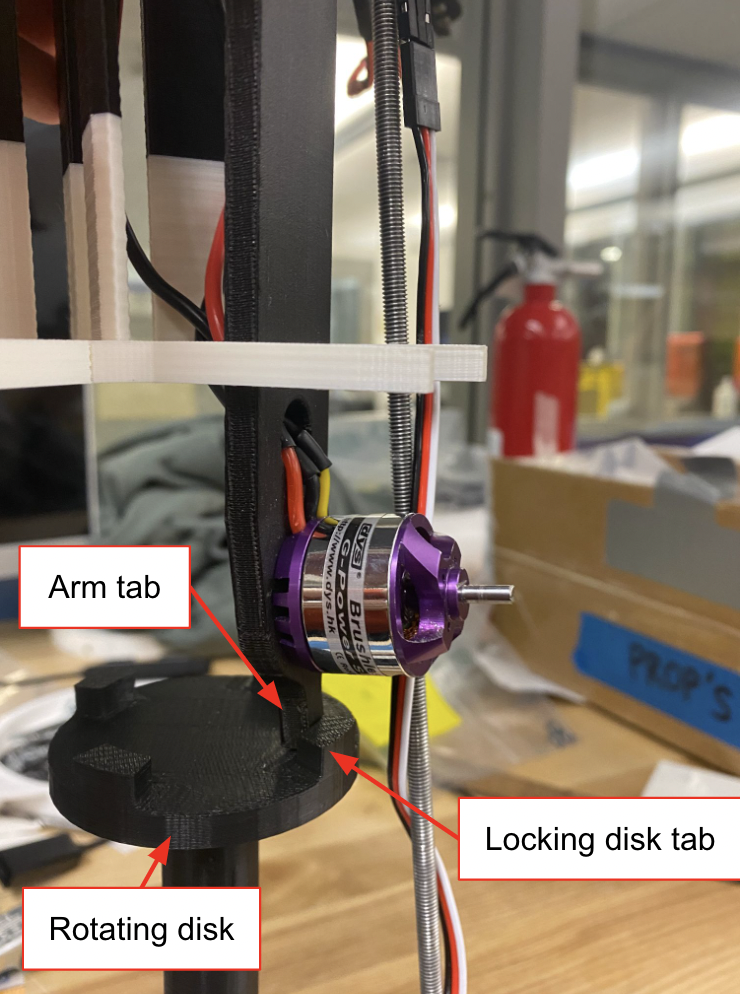
\includegraphics[width=0.6\textwidth]{src/figs/stowedarmlabeledview2.png}
    \caption{Stowed Arm in Locked Position}
    \label{fig:stowedarm}
\end{figure}

\subsection{Deployed Locking Mechanism}
Once the arms are outside of the rocket body, it is critical that they do not move around at all to prevent a moving center of thrust. To ensure that the propulsion arms remain in their fully deployed position, a deployed locking mechanism was developed. This mechanism involves a long-nose plunger spring pin which is mounted to the underside of the arm in a press-fit holder. The pin is compressed while inside the rocket but deploys into a small cutout when the arm has reached its deployed position to prevent it from falling below its fully deployed position. An image of this is shown in figure \ref{fig:deployedarm}.

\begin{figure}[H]
    \centering
    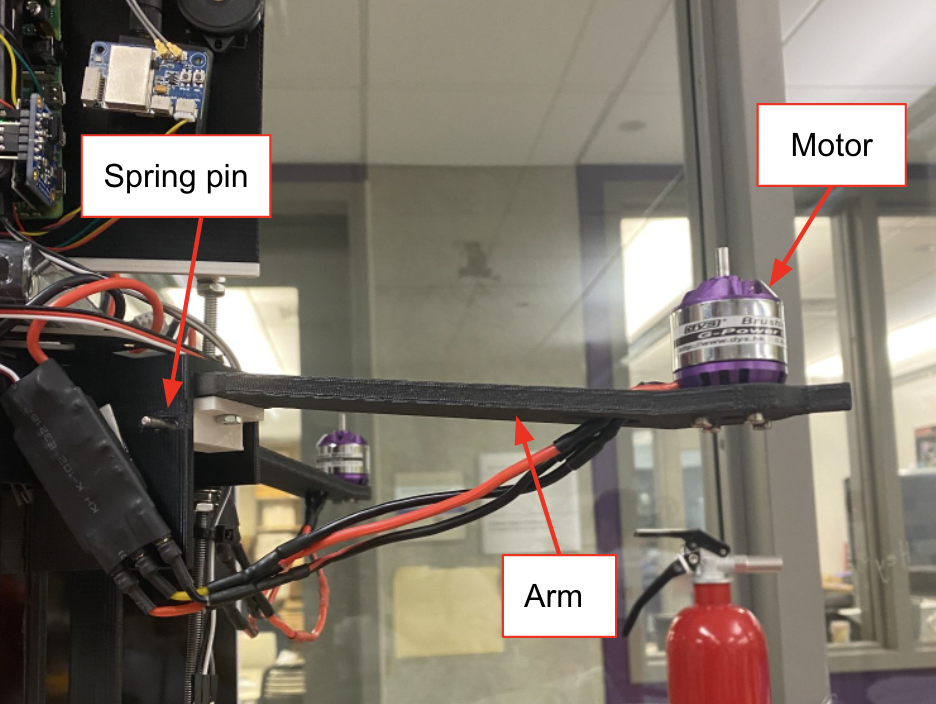
\includegraphics[width=0.9\textwidth]{src/figs/armdeployedlabeled.png}
    \caption{Deployed Arm with a Locking Mechanism}
    \label{fig:deployedarm}
\end{figure}

\subsection{Arm Core}
To facilitate the ability to remove all four arms at once for maintenance, they are all mounted to a centrally located 'arm core' as opposed to the actual rocket body. This component is mounted to the threaded rods via 8 nuts that are shouldered to prevent movement in the event of unusual flight attitude, vibration, and sudden acceleration. The arm core has four bays, one for each arm, that provide structures to support the deployment method, the propulsion arm, the deployed locking mechanism, the power distribution board (PDB), and the electronic speed controllers (ESCs).

Each arm is held in place by a 1/4" shoulder bolt that passes through both sides of the arm core bays, the arm, and the torsion springs. To support the torsion spring deployment method, each bay has a 30 degree slanted face that remains in contact with one end of the torsion springs. This face is slanted so that when the arm is fully deployed (a 90 degree offset from its stowed position), the 120 degree torsion spring is at its free angle. To help secure the torsion springs in their proper orientation, small tabs were added at the bottom of the slanted face to align the springs during assembly and prevent them from slipping out of place while compressed.

The top surface of the arm core is solid for two reasons. The primary reason for this design is to block the path of travel of the arm to prevent it from going beyond its fully deployed position and possibly having the propeller strike the rocket body. The secondary reason for this design is to provide a flat surface to which the PDB can mount.

Each bay also has two vertical walls on either side of the bay. These walls serve a variety of purposes. The primary purpose is to provide a surface to hold the deployed locking spring pin in its compressed position. The secondary purpose is to provide a flat mounting surface for the electronic speed controllers. One of these walls in each bay has a small cutout that allows the deployed locking spring pin to deploy into it when the arm reaches its fully deployed position, preventing the arm from moving below its deployed position. Extending below these main walls are two small structures that prevent the propeller from rotating inside the rocket body which could interfere with proper deployment.

\subsection{Propulsion Arm}
The propulsion arm is the primary component for this system but its design revolved heavily around the setup of the locking mechanisms and motor selection. 

At the end of the arm that attaches to the internal arm core, two protrusions are present that allow for the 1/4" shoulder bolt to pass through in order to securely attach to the arm core. Also, on this end of the arm are two small cutouts that extend 1.75" down the length of the arm. These cutouts provide a place for the torsion spring legs for deployment to slide into. This design ensures that the springs maintain their proper alignment while they are stowed. Finally, this end of the arm is also where the deployed locking spring pin attaches. This pin is connected via a press fit holder that is secured to the underside of the arm using counter-sunk through bolts. This pin holder also helps mechanically secure the springs to the arm, preventing them from disconnecting with the underside of the arm.

On the other end of the arm, 5 holes are included that provide mounts for the motor. Additionally, a small tab is present at the extreme of the arm. This tab is what interfaces with the pre-deployment locking mechanism to prevent the arm from inadvertently deploying before the landing system is called to action.

In order to accommodate the large motors required for the thrust needed, the arm has a 5/8" dip in it from the point it exits the rocket body to the point that the motor attaches. This dip was necessary to ensure that all components when stowed fit inside the confines of a 6" rocket body. 

\section{Landing Leg System Functionality} 
The landing legs support the rocket body upon landing and ensure that the rocket body lands upright in a stable position. The main components of this system are the primary and secondary strut which together distribute the loading upon landing impact, one locking mechanism to lock the leg in its stowed position, another single locking mechanism to lock the leg in the deployed position, and a deployment mechanism that provides the force to deploy the leg. This system is composed of 3 landing legs each spaced at 120 degrees from each other. Each landing leg is composed of the primary strut, secondary strut and supporting components, all of which are discussed below. All components with the exception of one are mounted to the outside of the rocket body using M3 bolts. To provide a flat mounting surface for the nut on the inside of the rocket, small internal mounts were printed that match the inner diameter of the tube on one side and are flat on the other. The bolt for each component passes through the component, the rocket body, then this part.

\subsection{Primary and Secondary Struts}
The landing leg uses a 2 strut system in which a primary and secondary strut are attached at the point that will contact the ground upon full deployment. When stowed both components run vertically up the side of the body tube. An image of the leg in the stowed position is shown in figure \ref{fig:LegStowed}. When deployed, they form a triangle that contacts the rocket in two places and the ground in one. The ends of the legs that attach to the rocket are also hinged using shoulder bolts to allow them to easily move to their deployed position when unlocked. The secondary strut is hinged in a fixed location at the very bottom end of the rocket body. In order to allow for the struts to move between their compact, stowed position along the sides of the rocket to their deployed position, a track and carriage system is needed. The primary strut is hinged to the carriage which has the ability to move up and down along the track mounted to the side of the rocket. The design of the track and carriage relied on the deployment method and locking mechanisms discussed below.

\begin{figure}[H]
    \centering
    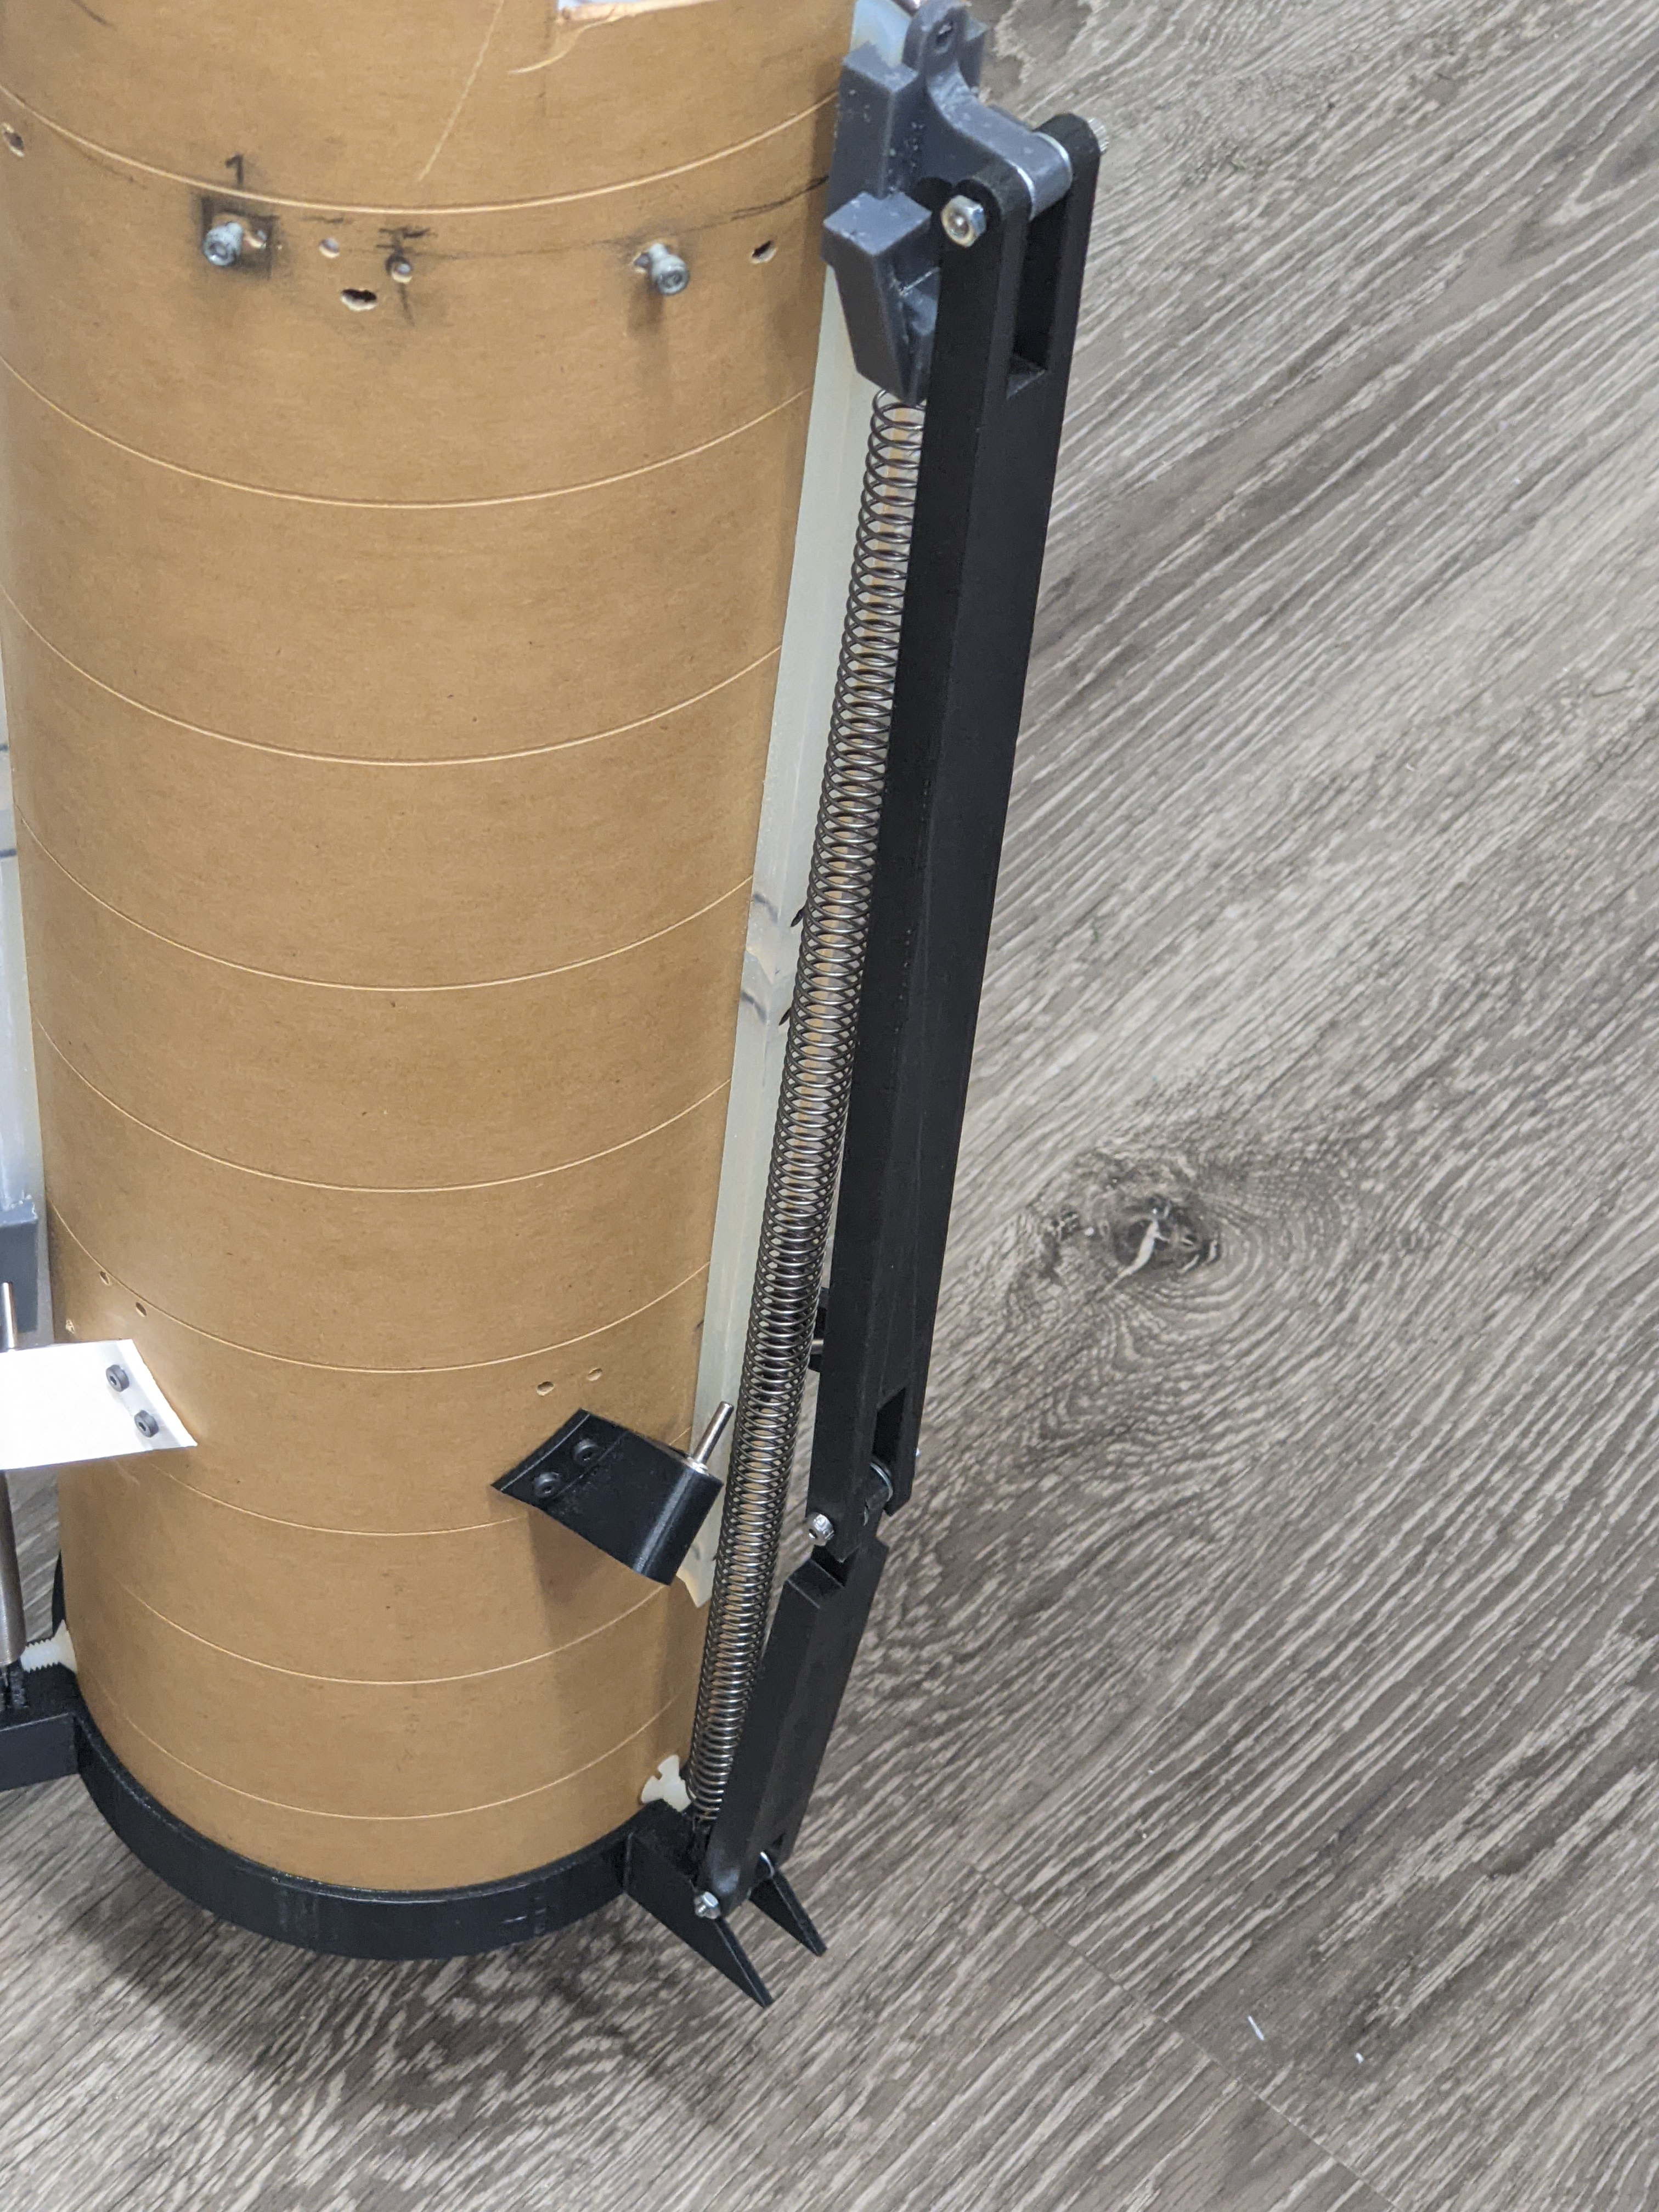
\includegraphics[width=0.5\textwidth]{src/figs/Stowed_Leg.jpg}
    \caption{Leg in Stowed Position}
    \label{fig:LegStowed}
\end{figure}

\subsection{Deployment Method}
Since the deployment relies on a track and carriage system, a linear spring was selected as the leg deployment mechanism. The spring attaches to the primary strut carriage at one end and a mount at the bottom of the rocket body at the other end. When fully stowed, the spring is pulling down on the carriage to bring it to its deployed position. Once fully deployed, the spring is still in a small amount of tension in order to keep force pulling the leg down and provide a small amount of suspension upon impact with the ground.

\subsection{Pre-Deployment Locking Mechanism}
To hold the leg in the stowed position, a pre-deployment locking mechanism is installed that restrains the motion of the carriage into its stowed position. This mechanism relies on the same servo as the propulsion arm pre-deployment locking mechanism. The mechanism consists of a 'spool' with three attach points. The spool is secured to the servo using a 50mm M3 bolt as well as cutout on its underside to prevent the spool from slipping (figure \ref{fig:spoolc}). The propulsion arm 'disk' is attached to this spool by sliding over it and then being secured with M2 screws in threaded inserts. Attached to the spool at the 3 attach points are pins pass through the rocket body and into the back of the carriage. When the spool is rotated, these pins are pulled out of the back of the carriage, allowing it to be pulled into the deployed position by the attached linear spring. 

\begin{figure}[H]
    \centering
    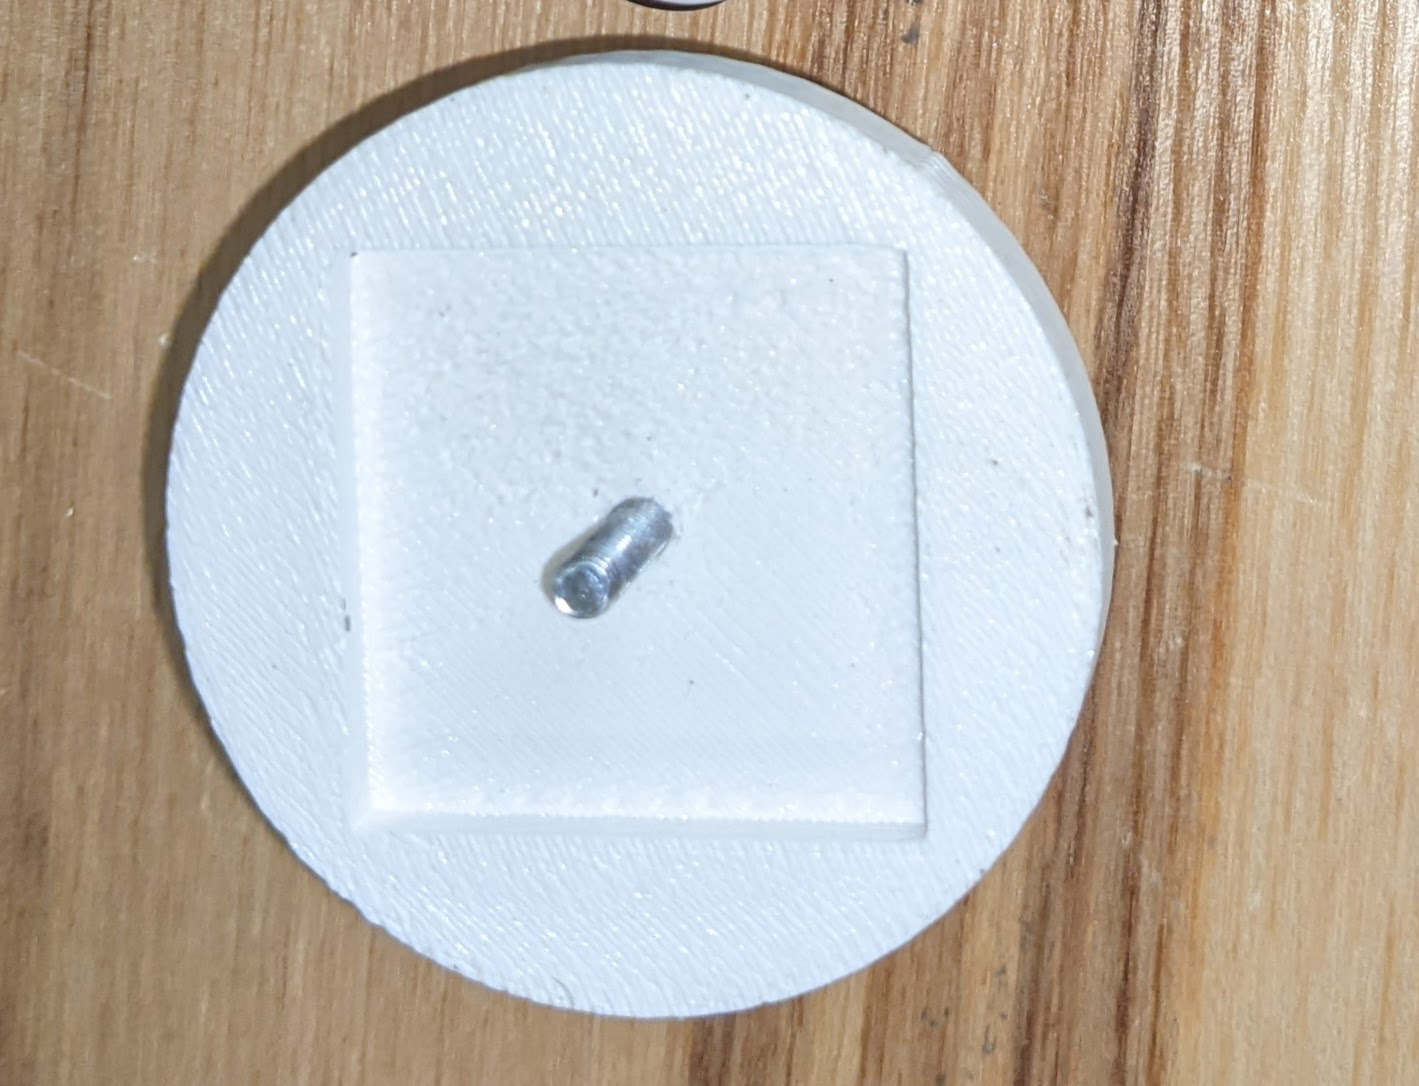
\includegraphics[width=0.5\textwidth]{src/figs/Spool_Cutout.jpg}
    \caption{Cutout Underneath Spool}
    \label{fig:spoolc}
\end{figure}

\subsection{Deployed Locking Mechanism}
Once fully deployed, a pair of spring pins holds each landing leg in its fully deployed position. Both pins are mounted just above the carriages fully deployed position facing slightly upwards. As the carriage is pulled past them, they compress, allowing the carriage to pass. Once the carriage has passed the pins, they return to their extended position which blocks the carriage from being able to slide back up the track when weight is placed on the landing legs. An image of the pin inside the core is shown in figure \ref{fig:pin_rocket}.

\begin{figure}[H]
    \centering
    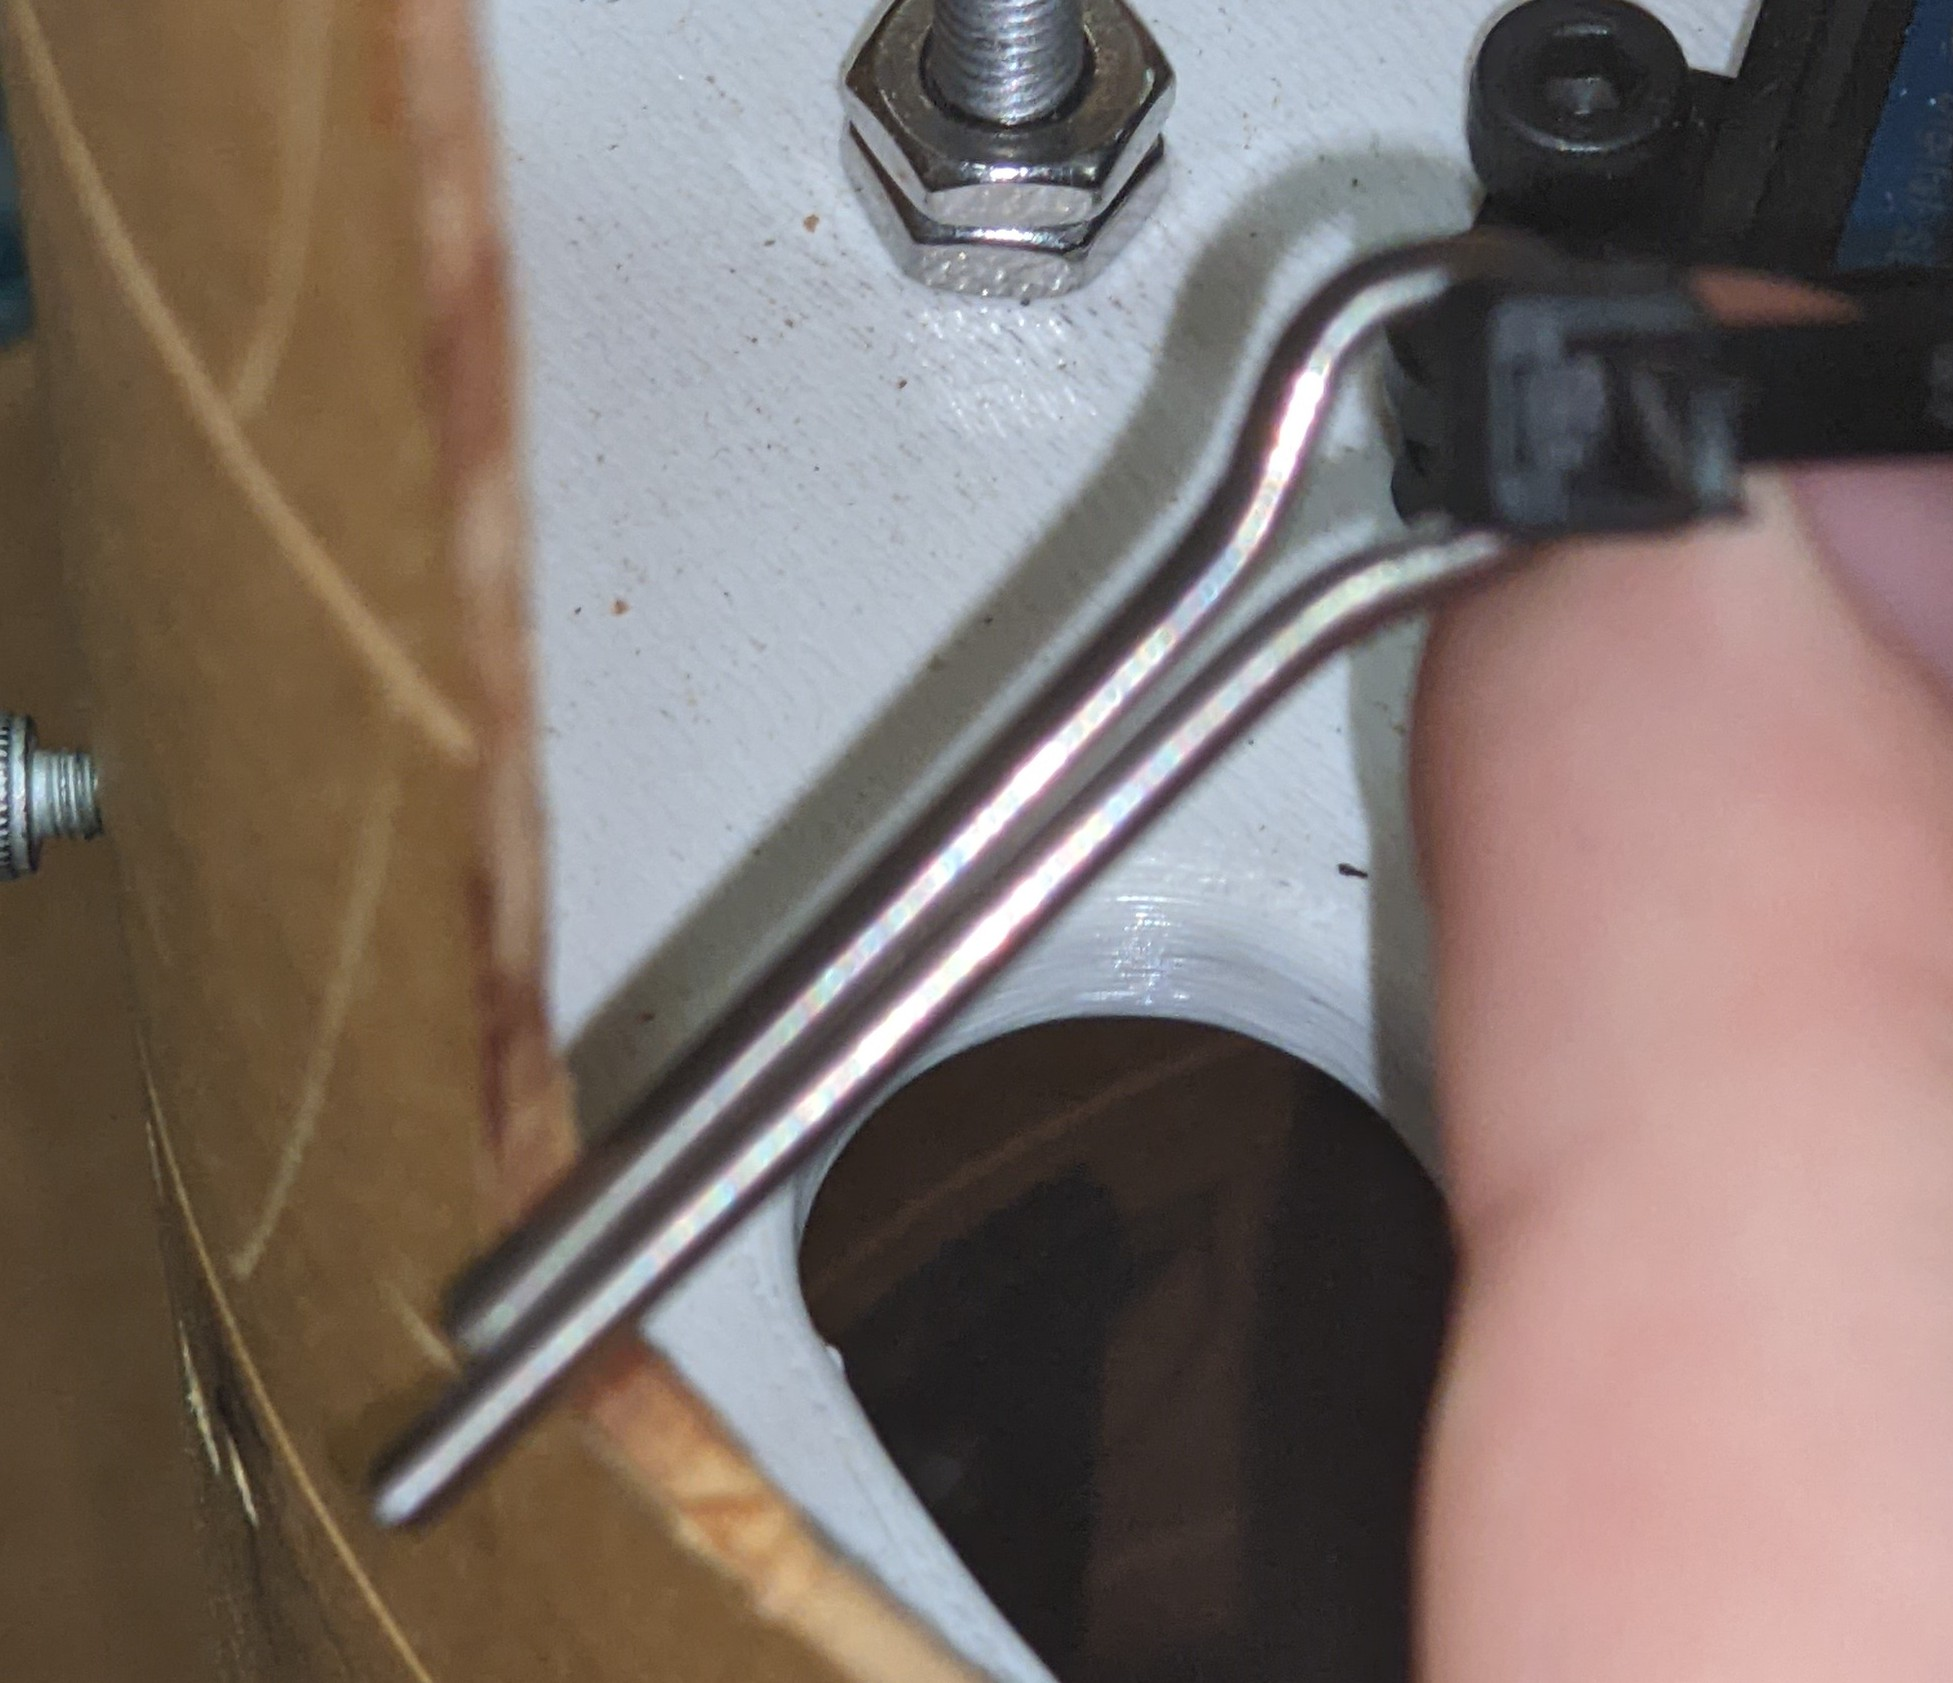
\includegraphics[width=0.5\textwidth]{src/figs/Pins_Rocket.jpg}
    \caption{Pins to Stow Rocket}
    \label{fig:pin_rocket}
\end{figure}

\subsection{Track and Carriage}
The track and carriage are designed to function without the use of any form of bearing or lubrication. They use a nested design in which the track mounts to the rocket body and the carriage is shaped so that it is constrained to only motion in the direction necessary with small clearance for very minor side to side movement (figure \ref{fig:CLB}). 

\begin{figure}[H]
    \centering
    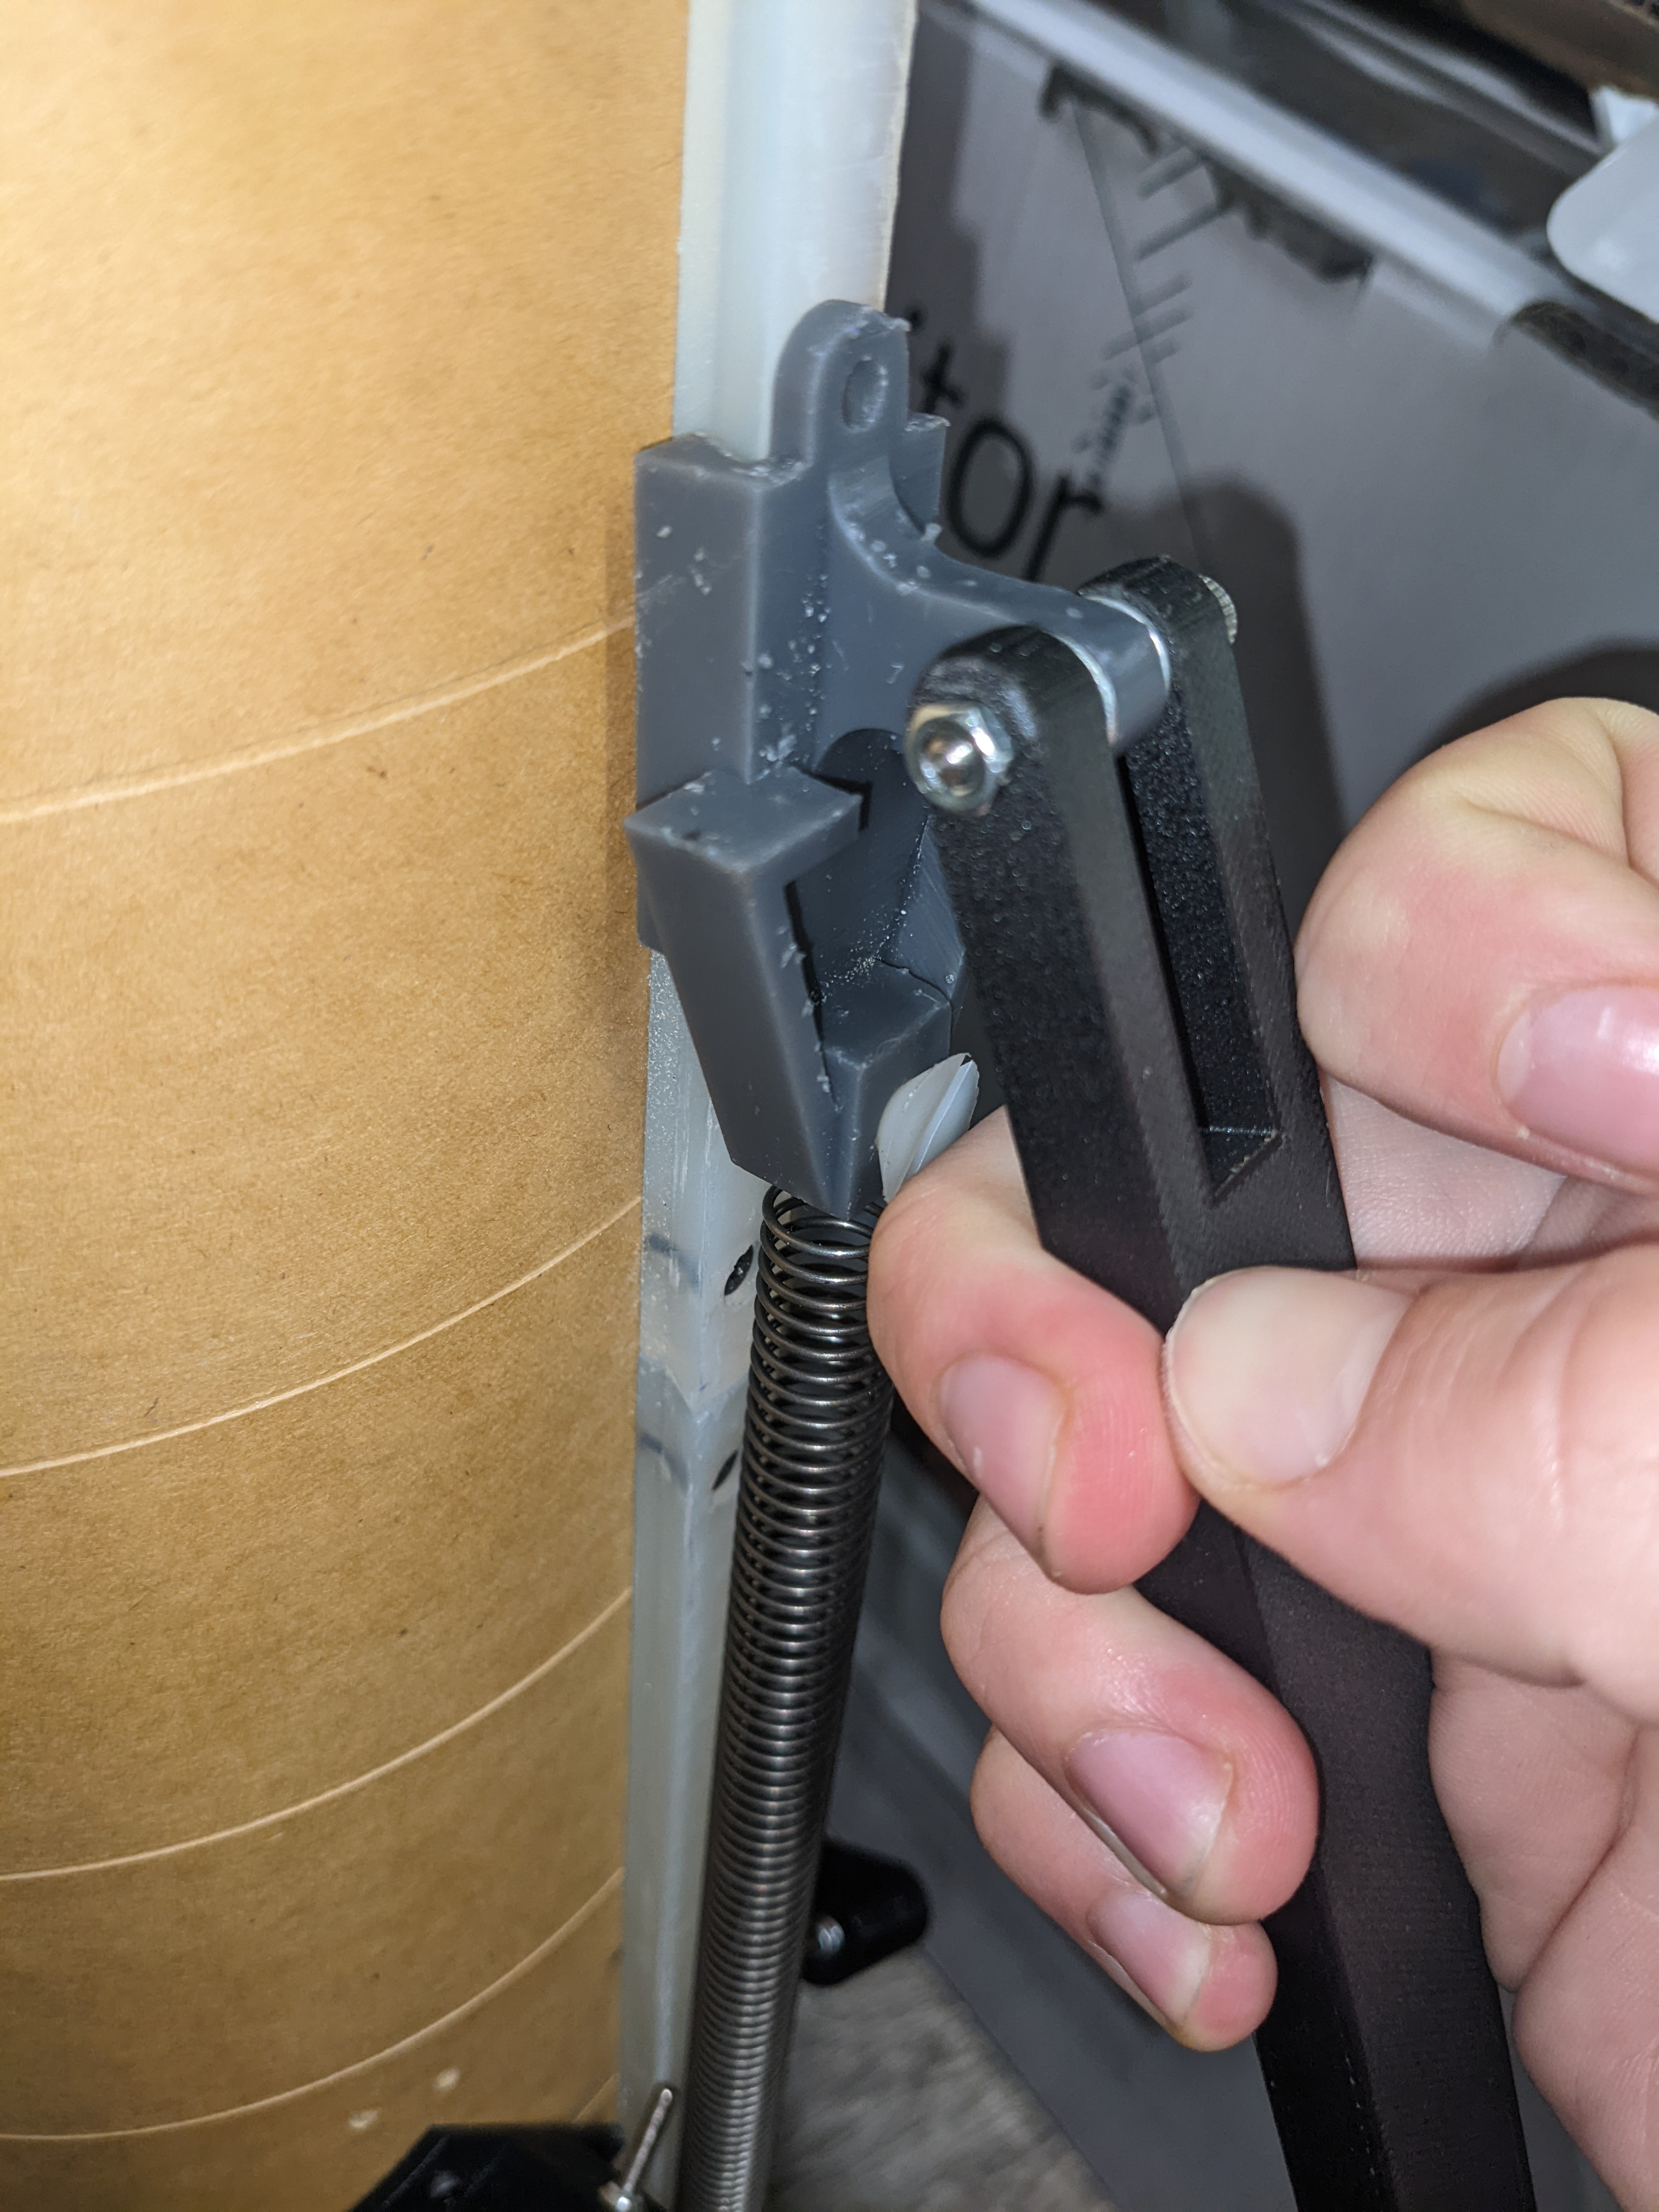
\includegraphics[width=0.35\textwidth]{src/figs/Carriage_Leg.jpg}
    \caption{Carriage on Leg Bracket}
    \label{fig:CLB}
\end{figure}

The carriage has an attach point for the primary strut that protrudes from the carriage surface. Additionally, a mount point for the upper end of the spring is present. The spring goes into the slot in the carriage and is secured by a plastic screw that passes through the carriage and center of the spring hook. A small protrusion and hole is added to the very top of the carriage through which the pin for the pre-deployment locking mechanism passes. On the sides of the carriage, angled walls are present to push the deployed locking pins into their housing while the carriage passes. Just beyond these angled walls, the carriage narrows, providing a contact surface for the deployed locking pins and the carriage.

\subsection{Secondary Strut Support}
To prevent the landing leg system from traveling beyond its ideal deployed angle of 40 degrees (see Section \ref{ea:landing-legs}), a lower support is in place that stops the secondary strut from travelling beyond 135 degrees from its stowed position. This support is one ring that contains an angled surface for each leg set. The ring not only helps with alignment since all three leg supports are mounted together, but also distributing the load of impact around a larger area of the body tube to minimize the risk of component failure. On each of the support faces is a hinge point for the secondary strut as well as an attachment point for the lower end of the deployment spring. The spring here is also held in place through the use of a through screw that is constrained from coming out by the screw head as well as the rocket body.